\documentclass{article}
\usepackage[margin=0.25in]{geometry}
\usepackage{pdflscape}
\usepackage{amssymb}
\usepackage{xcolor}
\usepackage{tikz}
\usetikzlibrary{positioning, shapes.geometric}

% Define custom colors
\definecolor{darkblue}{RGB}{25,25,112}
\definecolor{lightblue}{RGB}{173,216,230}
\definecolor{darkred}{RGB}{139,0,0}
\definecolor{darkgreen}{RGB}{0,100,0}
\definecolor{purple}{RGB}{128,0,128}

\begin{document}
\thispagestyle{empty}
\begin{landscape}

\begin{center}
{\Huge\bfseries\color{darkblue} DEFEAT THE FIRST ORDER}\\[0.5cm]
{\Large\itshape A Choose Your Own Adventure Decision Tree}
\end{center}

\vspace{1cm}

\resizebox{1.3\textwidth}{!}{
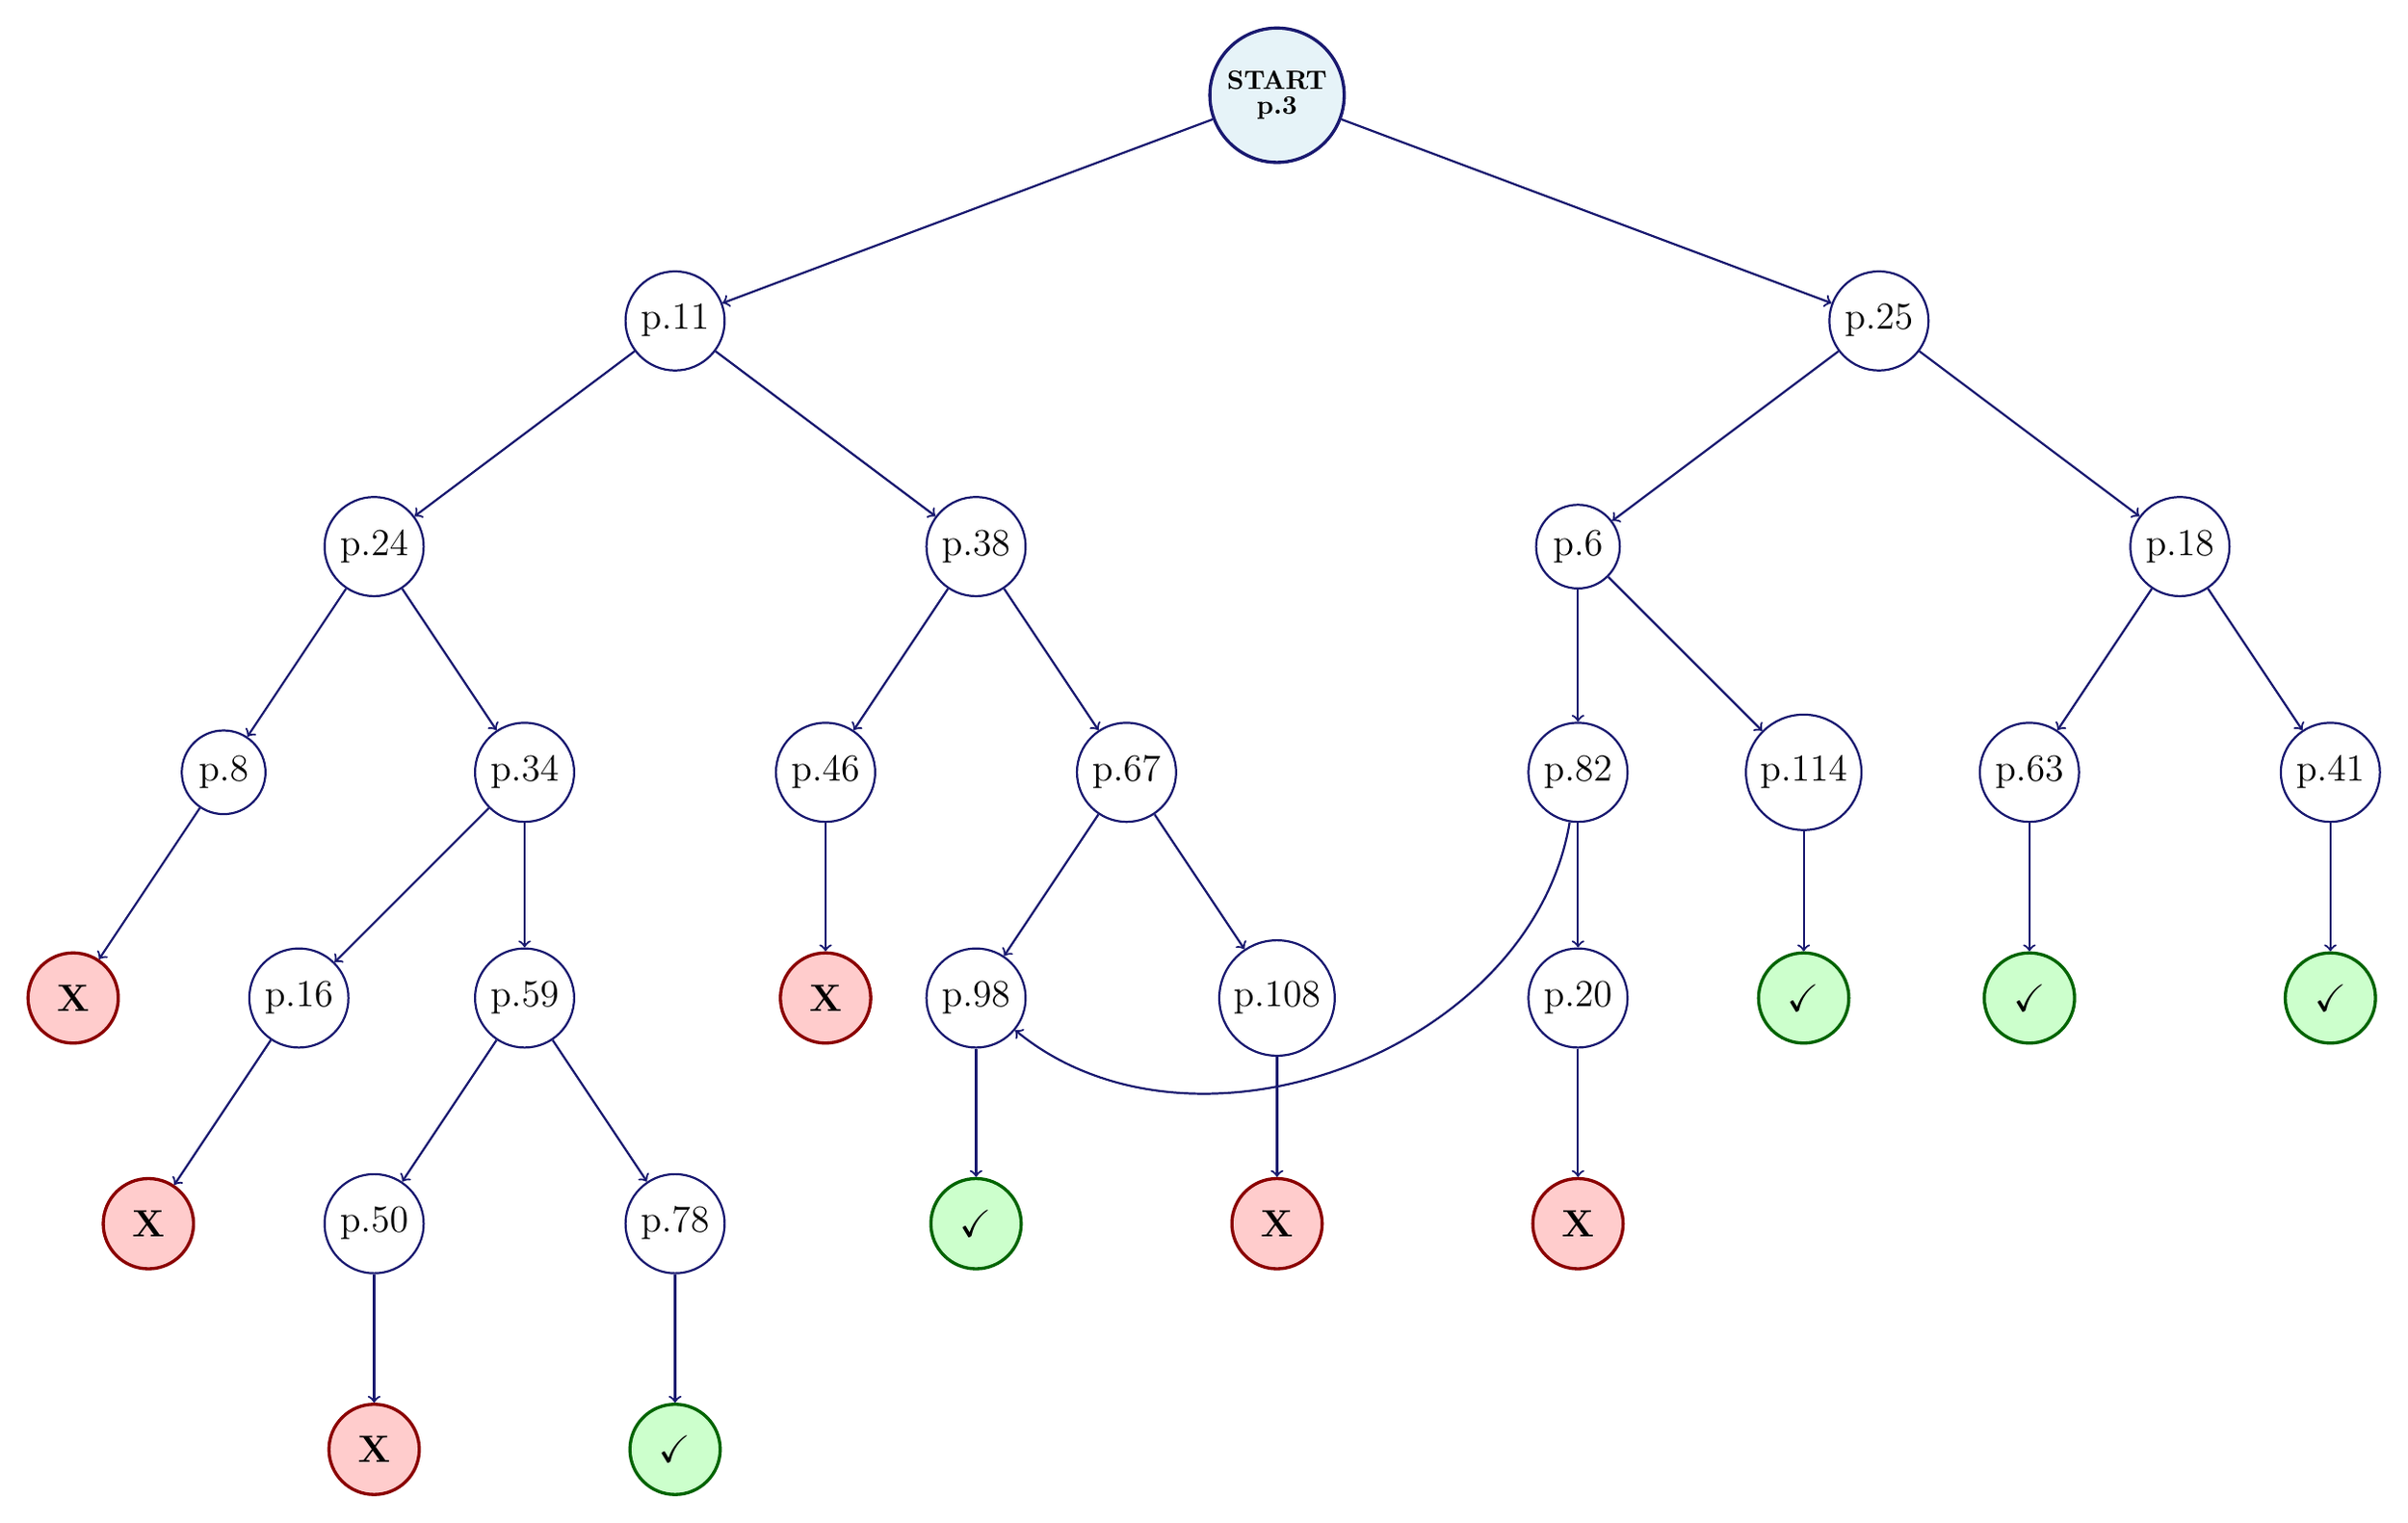
\begin{tikzpicture}[
    % Node styles
    start/.style={circle, draw=darkblue, fill=lightblue!30, minimum size=16mm, very thick, font=\bfseries},
    page/.style={circle, draw=darkblue, minimum size=10mm, thick, font=\Large},
    success/.style={circle, draw=darkgreen, fill=green!20, minimum size=12mm, very thick, font=\bfseries},
    failure/.style={circle, draw=darkred, fill=red!20, minimum size=12mm, very thick, font=\bfseries},
    repeat/.style={diamond, draw=purple, fill=purple!20, minimum size=10mm, thick, font=\scriptsize},
    % Edge styles
    edge/.style={draw=darkblue, thick, ->}
]

% Level 0 - Start
\node[start] (start) at (0,0) {\shortstack{START\\p.3}};

% Level 1
\node[page] (p11) at (-8,-3) {p.11};
\node[page] (p25) at (8,-3) {p.25};

% Level 2 - Left branch from p.11
\node[page] (p24) at (-12,-6) {p.24};
\node[page] (p38) at (-4,-6) {p.38};

% Level 2 - Right branch from p.25
\node[page] (p6) at (4,-6) {p.6};
\node[page] (p18) at (12,-6) {p.18};

% Level 3 - From p.24
\node[page] (p8) at (-14,-9) {p.8};
\node[page] (p34) at (-10,-9) {p.34};

% Level 3 - From p.38
\node[page] (p46) at (-6,-9) {p.46};
\node[page] (p67) at (-2,-9) {p.67};

% Level 3 - From p.6
\node[page] (p82) at (4,-9) {p.82};
\node[page] (p114) at (7,-9) {p.114};

% Level 3 - From p.18
\node[page] (p41) at (14,-9) {p.41};
\node[page] (p63) at (10,-9) {p.63};

% Level 3 - From p.8
\node[failure] (x8) at (-16,-12) {\Large X};

% Level 3 - From p.34
\node[page] (p16) at (-13,-12) {p.16};
\node[page] (p59) at (-10,-12) {p.59};

% Level 4 - From p.16
\node[failure] (x16) at (-15,-15) {\Large X};

% Level 4 - From p.59
\node[page] (p50) at (-12,-15) {p.50};
\node[page] (p78) at (-8,-15) {p.78};

% Level 4 - From p.46
\node[failure] (x1) at (-6,-12) {\Large X};

% Level 4 - From p.67
\node[page] (p98) at (-4,-12) {p.98};
\node[page] (p108) at (0,-12) {p.108};

% Level 4 - From p.82
\node[page] (p20) at (4,-12) {p.20};

% Level 4 - From p.114
\node[success] (win114) at (7,-12) {\Large $\checkmark$};

% Level 4 - From p.41
\node[success] (win41) at (14,-12) {\Large $\checkmark$};

% Level 4 - From p.63
\node[success] (win63) at (10,-12) {\Large $\checkmark$};

% Level 5 - From p.50
\node[failure] (x50) at (-12,-18) {\Large X};

% Level 5 - From p.78
\node[success] (win78) at (-8,-18) {\Large $\checkmark$};

% Level 5 - From p.98
\node[success] (win98) at (-4,-15) {\Large $\checkmark$};

% Level 5 - From p.108
\node[failure] (x108) at (0,-15) {\Large X};

% Level 5 - From p.20
\node[failure] (x3) at (4,-15) {\Large X};




% Draw all edges
\draw[edge] (start) -- (p11);
\draw[edge] (start) -- (p25);

\draw[edge] (p11) -- (p24);
\draw[edge] (p11) -- (p38);

\draw[edge] (p25) -- (p6);
\draw[edge] (p25) -- (p18);

\draw[edge] (p24) -- (p8);
\draw[edge] (p24) -- (p34);

\draw[edge] (p8) -- (x8);

\draw[edge] (p34) -- (p16);
\draw[edge] (p34) -- (p59);

\draw[edge] (p38) -- (p46);
\draw[edge] (p38) -- (p67);

\draw[edge] (p18) -- (p41);
\draw[edge] (p18) -- (p63);

\draw[edge] (p6) -- (p82);
\draw[edge] (p6) -- (p114);

\draw[edge] (p46) -- (x1);

\draw[edge] (p41) -- (win41);
\draw[edge] (p63) -- (win63);

\draw[edge] (p67) -- (p98);
\draw[edge] (p67) -- (p108);

\draw[edge] (p82) to [bend left=60] (p98);
\draw[edge] (p82) -- (p20);

\draw[edge] (p114) -- (win114);

\draw[edge] (p98) -- (win98);

\draw[edge] (p108) -- (x108);

\draw[edge] (p16) -- (x16);

\draw[edge] (p59) -- (p50);
\draw[edge] (p59) -- (p78);

\draw[edge] (p50) -- (x50);
\draw[edge] (p78) -- (win78);

\draw[edge] (p20) -- (x3);

\end{tikzpicture}
}

\end{landscape}
\end{document}